\chapter{Background}
\label{background}

\section{RoboCup Competition}

The RoboCup Competition, in its short history, has grown to a well-established annual event bringing together the best robotics researchers from all over the world. The initial conception by Hiroaki Kitano~\cite{robocup} in 1993 led to the formation of the RoboCup Federation with a bold vision: ``By the year 2050, to develop a team of fully autonomous humanoid robots that can win against the human world soccer champions''.The uniqueness of RoboCup stems from the real-world challenge it poses, whereby the core problems of robotics (perception, cognition, action, coordination) must be addressed simultaneously under real-time constraints. The proposed solutions are tested on a common benchmark environment through soccer games in various leagues,with the goal of promoting the best approaches, and ultimately advancing the state-of-the-art in the area. 

\section{RoboCup Leagues}

Beyond soccer, RoboCup now includes also competitions in search-and-rescue missions (RoboRescue), home-keeping tasks (RoboCup@Home), robotic performances (RoboDance), and simplified soccer leagues for K-12 students (RoboCup Junior). Broadening the research areas where RoboCup focuses, was a very interesting and clever addition, which enables all the more scientists and researchers combine their expertise in order to solve real world problems. A lot of progress has been made so far in many disciplines of robotics and RoboCup has been established in one of the most important events around the world.

\section{RoboRescue}

RoboRescue initiated from the need of people to create robots capable of operating in hostile or inaccessible environments by humans. This area is very motivating in terms of helping the humanity while promoting robotics. Multi-agent team work coordination, physical robotic agents and rescue strategies are all being tested in real or simulated environments (Figure~\ref{fig:roboRescue}), using sensors including cameras, temperature sensors, $CO_2$ sensors and other that allow for fast and efficient human body localization.

\begin{figure}[h]
	\begin{center}
		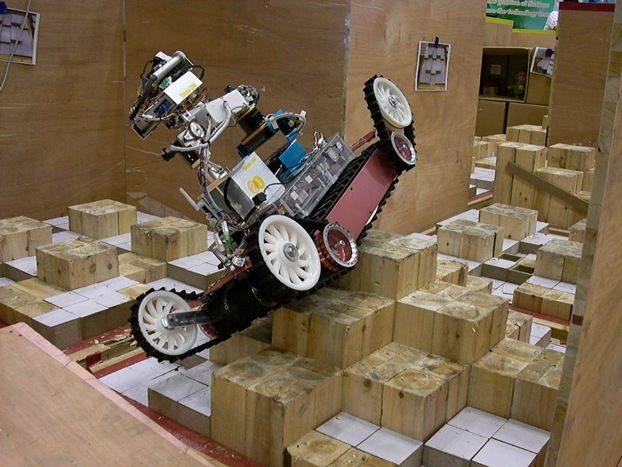
\includegraphics[height = 6cm]{Chapter1/figures/roboRescue.jpeg}
 		\caption{RoboRescue environments can become extremely hostile for robots.}
 		\label{fig:roboRescue}
	\end{center}
\end{figure}

\section{RoboCup@Home}

The RoboCup@Home league aims to develop service and assistive robot technology with high relevance for future personal domestic applications. It is the largest international annual competition for autonomous service robots and is part of the RoboCup initiative. A set of benchmark tests is used to evaluate the robots' abilities and performance in a realistic non-standardized home environment setting (Figure~\ref{fig:robocup@home}).

Most of the research lies in many domains including Human-Robot-Interaction and Cooperation, Navigation and Mapping in dynamic environments, Computer Vision and Object Recognition under natural light conditions, Object Manipulation, Adaptive Behaviors, Behavior Integration, Ambient Intelligence, Standardization and System Integration.

\begin{figure}[h]
	\begin{center}
		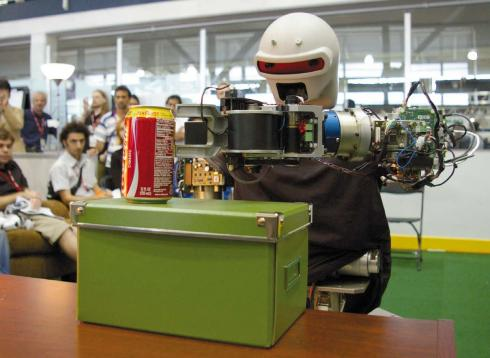
\includegraphics[height = 6cm]{Chapter1/figures/robocup@home.jpeg}
 		\caption{Robocup@Home represents a social aspect of robotics interacting with people.}
 		\label{fig:robocup@home}
	\end{center}
\end{figure}


\section{RoboCup Junior}

Robocup Junior is one of the smaller and less competitive, in terms of antagonism sub-domain of RoboCup, which is mainly intended in the preparation of gifted children interested in robotics. It is very important to understand that this competition has nothing to be jealous of the other leagues, but in fact share the same vision and the required dedication to excel.

\subsection{Dance}

RoboDance might one say to be the most amusing competition of RoboCup, where robots are performing in front of their audience. Dances, most of times, are innovative and unique. Developers are being judged on the novelty of motions, the cooperation of the robots, and finally the synchronization of the robot motion according to the music.

\subsection{Rescue}

Rescue in the Junior league, is a simplified version of RoboRescue and is limited in the line-following problem. Each team has to qualify from a number of tracks whose difficulty gradually increases. The trials are judged on the duration of the track completion and on the agent's behavior in misleading parts of the track, such as line intersections, or line gaps.

\subsection{Soccer}

The soccer competition is played by two cylindrical robots which share the same features and play soccer in a box or in a table surrounded by low walls. This is by far the most exciting competition in Robocup Junior and the most demanding.


\section{RoboCup Soccer League}

The RoboCup Soccer League, is the domain with the most fans. In this league researchers combine their technical knowledge in order to prepare the best robotic soccer team among other universities.

\subsection{The Standard Platform League}

Standard Platform League (SPL) of the RoboCup competition is the most popular league, featuring two to four humanoid Aldebaran Nao robot players in each team. This league was formerly known as the Four-Legged League with Sony Aibo robots, which were replaced in 2008 by Aldebaran Nao (Figure~\ref{fig:spl}). Games take place in a $4 m \times 6 m$ field marked with thick white lines on a green carpet. The two colored goals (sky-blue and yellow) also serve as landmarks for localizing the robots in the field. Each game consists of two 10-minute halves and teams switch colors and sides at halftime. There are several rules enforced by human referees during the game. For example, a player is punished with a 30-seconds removal from the field if he performs an illegal action, such as pushing an opponent for more than three seconds, grabbing the ball between his legs for more than three seconds, or entering his own goal area as a defender.

\begin{figure}[h]
	\begin{center}
		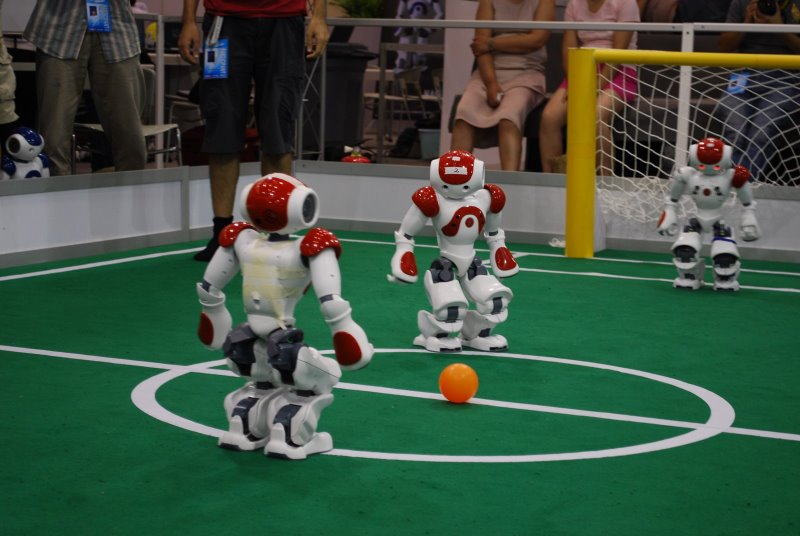
\includegraphics[height = 8cm]{Chapter1/figures/spl.jpg}
 		%\caption{Middle size league teams preparing before a game in RoboCup German Open 2007.}
		\caption{Standard Platform League game in Robocup 2008( Opponents should be in different colors, but there was a lack of Nao robots in that event due to malfunctions )}
 		\label{fig:spl}
	\end{center}
\end{figure}


The main characteristic of the Standard Platform League is that no hardware changes are allowed; all teams use the exact same robotic platform and differ only in terms of their software. This convention results to the league's enrichment of a unique set of features: autonomous player operation, vision-based perception, legged locomotion and action. Given that the underlying robotic hardware is common for all competing teams, research effort has been focused on the development of more efficient algorithms and techniques for visual perception, active localization, omni-directional motion, skill learning, and coordination strategies. During the course of the years, one could easily notice a clear progress in all research directions.

\subsection{Simulation League}

Every year there is a number of simulation games taking place in RoboCup competitions. These include 2D soccer games, where teams consist of 11 agents providing to developers with a perfect multi-agent environment to tune and benchmark their solutions. 3D simulation games exist as well; usage of physics engines demand more realistic approaches.

Simulators offer the ability to control the amount of ``negative'' realism added in these environments; thus, it is a great way to allow researchers work focusing in multi-agent cooperation approaches and other state-of-the-art algorithms, abstracting from real-world problems (gravity, forces etc).

In RoboCup 2008, three of the most important simulation leagues, were the official RoboCup Simulation League run in an open source simulator, the Microsoft Robotics Studio competition, and the Webots RoboStadium.

\subsection{Small Size League}

A Small Size robot soccer game takes place between two teams of five robots each. Each robot must fit within an 180mm diameter circle and must be no higher than 15cm, unless they use on-board vision. Robots play soccer on a 6.05m long by 4.05m wide, green carpeted field with an orange golf ball. Vision information is either processed on-board the robot or is transmitted back to the off-field PC. Another off-field PC is being used to communicate referee commands and position information to the robots, when an extra camera mounted on top of the field serves as the vision sensor. Typically, off-field PCs are used in the coordination and control of the robots. Communication is wireless and typically use dedicated commercial FM transmitter/receiver units\footnote{http://small-size.informatik.uni-bremen.de/rules:main}.

\subsection{Middle Size League}

Middle Size is more competitive and demanding, having the largest field dimensions among other leagues (Figure~\ref{fig:middleSize}). Two teams of mid-sized robots consist of 5 players each, with all sensors on-board play soccer on a field of $18 m \times 12 m$, whereas relevant objects are distinguished by colors only. Communication among robots (if any) is supported on wireless communications. Once again, no external intervention by humans is allowed, except to insert or remove robots in/from the field. These robots are the best players far among other leagues. The robots' bodies are heavy enough having powerful motors, heavy batteries, omni-directional camera, and a full laptop computer running in every robot; characteristics that make this league a great domain for research.


\begin{figure}[h]
	\begin{center}
		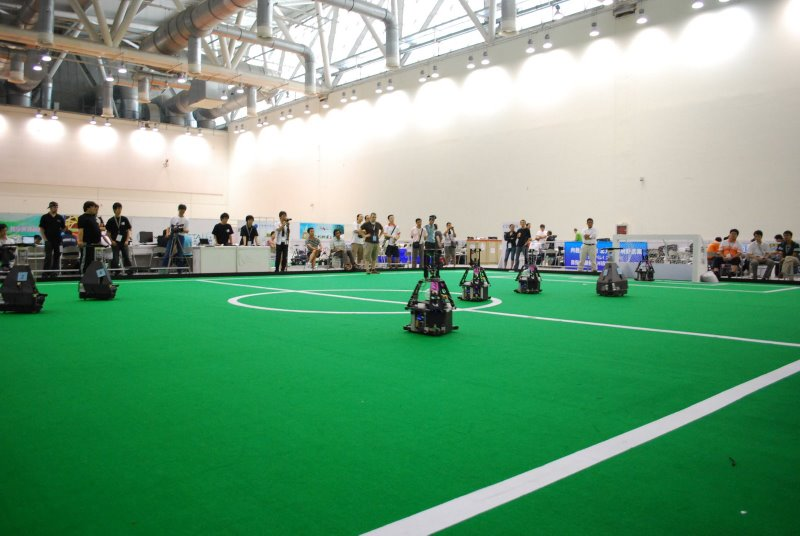
\includegraphics[height = 8cm]{Chapter1/figures/middleSize1.jpg}
 		%\caption{Middle size league teams preparing before a game in RoboCup German Open 2007.}
		\caption{Middle size league game in Robocup 2008.}
 		\label{fig:middleSize}
	\end{center}
\end{figure}

\subsection{Humanoid League}

The Humanoid League is one of the most dynamically progressing leagues and the one closest to the 2050's goal. In this league, autonomous robots with a human-like body plan and human-like senses play soccer against each other. In addition to soccer competitions, technical challenges take place. The robots are divided into two size classes: KidSize (30-60cm height) and TeenSize (100-160cm height). Dynamic walking, running, and kicking the ball while maintaining balance, visual perception of the ball, other players, and the field, self-localization, and team play are among the many research issues investigated in this league. Several of the best autonomous humanoid robots in the world compete in the RoboCup Humanoid League\footnote{http://www.tzi.de/humanoid/bin/view/Website/WebHome}.